% What the canonical serialisation buys: the hash fixes the claim, not one
% spelling of it. Hashes are the values the implementation actually produces.
\documentclass[tikz,border=3mm]{standalone}
\usepackage{tikz}
\usetikzlibrary{arrows.meta,positioning,calc,fit}

\definecolor{ink}{HTML}{1A1A1A}
\definecolor{accent}{HTML}{8C1D18}
\definecolor{mute}{HTML}{9E9E9E}

\begin{document}
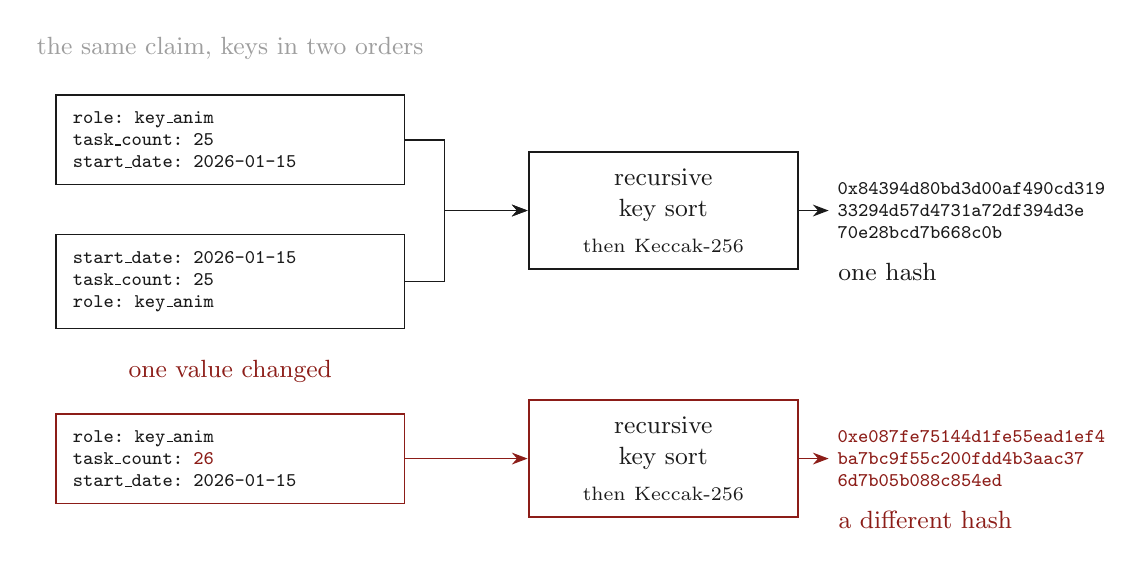
\begin{tikzpicture}[
  font=\rmfamily, ink,
  rec/.style={draw=ink, line width=0.5pt, align=left, inner sep=6pt,
              font=\scriptsize\ttfamily, text width=4.0cm},
  op/.style={draw=ink, line width=0.7pt, align=center, inner sep=6pt,
             font=\small, text width=3.0cm},
  hash/.style={align=left, font=\scriptsize\ttfamily, inner sep=3pt},
  fwd/.style={-{Stealth[length=2mm]}, draw=ink, line width=0.6pt},
]

% ---- two spellings of the same claim ---------------------------------------
\node[rec] (a) at (0,1.05) {
  role: key\_anim\\
  task\_count: 25\\
  start\_date: 2026-01-15
};
\node[rec] (b) at (0,-0.75) {
  start\_date: 2026-01-15\\
  task\_count: 25\\
  role: key\_anim
};
\node[font=\small, anchor=south, text=mute] at (0,1.95)
  {the same claim, keys in two orders};

% ---- the operation ----------------------------------------------------------
\node[op] (canon) at (5.5,0.15) {recursive\\key sort\\[2pt]
  {\scriptsize then Keccak-256}};
\draw[fwd] (a.east) -- ++(0.5,0) |- (canon.west);
\draw[fwd] (b.east) -- ++(0.5,0) |- (canon.west);

% ---- one hash ---------------------------------------------------------------
\node[hash, anchor=west] (h1) at (7.6,0.15)
  {0x84394d80bd3d00af490cd319\\33294d57d4731a72df394d3e\\70e28bcd7b668c0b};
\draw[fwd] (canon.east) -- (h1.west);
\node[font=\small, anchor=north west, text=ink] at ($(h1.south west)+(0,-0.08)$)
  {one hash};

% ---- a changed claim --------------------------------------------------------
\node[rec, draw=accent] (c) at (0,-3.0) {
  role: key\_anim\\
  task\_count: \textcolor{accent}{\textbf{26}}\\
  start\_date: 2026-01-15
};
\node[font=\small, anchor=south, text=accent] at (0,-2.15)
  {one value changed};
\node[op, draw=accent] (canon2) at (5.5,-3.0) {recursive\\key sort\\[2pt]
  {\scriptsize then Keccak-256}};
\draw[fwd, draw=accent] (c.east) -- (canon2.west);
\node[hash, anchor=west, text=accent] (h2) at (7.6,-3.0)
  {0xe087fe75144d1fe55ead1ef4\\ba7bc9f55c200fdd4b3aac37\\6d7b05b088c854ed};
\draw[fwd, draw=accent] (canon2.east) -- (h2.west);
\node[font=\small, anchor=north west, text=accent]
  at ($(h2.south west)+(0,-0.08)$) {a different hash};

\end{tikzpicture}
\end{document}
